\section{概要}

この「お絵描きAI」では、人間が途中まで書いた絵をもとに、完成形を予測して残りの部分を描き足すモデルの作成を目指しました。学習データとして、Googleが提供する Quick Draw!\cite{quickdraw}のデータセットを使用しました。このデータセットは、ユーザーが指定されたお題に対して20秒以内に絵を描き、それをAIが判定するというウェブアプリから収集されたものです。全345クラス、合計5000万件以上のスケッチデータが含まれており、それぞれが連続する点の座標データとして記録されています。これを基に、点群、画像、系列データの各アプローチからモデル構築を試みました。

\section{点群}
\subsection{実験}
Quick Draw!\cite{quickdraw}のデータ形式が連続する点による表現であるため、絵の描き順に依らない点群としてのアプローチが有効だと考え、エンコーダとしてPointNet\cite{pointnet}を用いたモデルを構築しました。PointNet\cite{pointnet}とは、3次元点群データを処理するために提案されたモデルであり、各点を個別に処理した後に、Max Poolingを用いることで点群の持つ順序に依存しない特徴量を抽出するモデルです。デコーダとして、線形層による固定長の点群生成や、LSTM・Transformerによる逐次生成などを試しました。しかし、どの手法も生成された点群はまばらで、図\ref{fig:pointnet_output}のように絵に見えるような点群を生成することはできませんでした。生成モデルとしてGANやDiffusionモデルも試しましたが、期待する結果を得ることはできませんでした。特にGANでは、Discriminatorと比較してGeneratorの性能がとても低く、どれだけDiscriminatorの性能を落としてもDiscriminatorが勝ってしまい学習が進みませんでした。

\begin{figure}[h]
  \begin{minipage}[b]{0.45\linewidth}
    \centering
    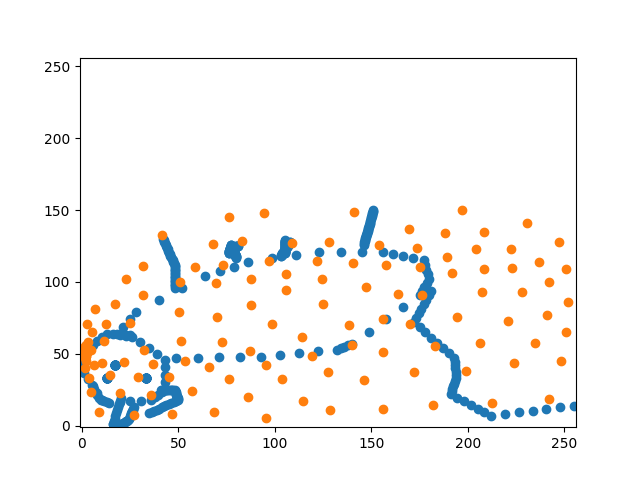
\includegraphics[keepaspectratio, scale=0.45]{draw-forecast/fig/pointnet_output1.png}
    \subcaption{全データ}
    \label{fig:pointnet_output}
  \end{minipage}
  \begin{minipage}[b]{0.45\linewidth}
    \centering
    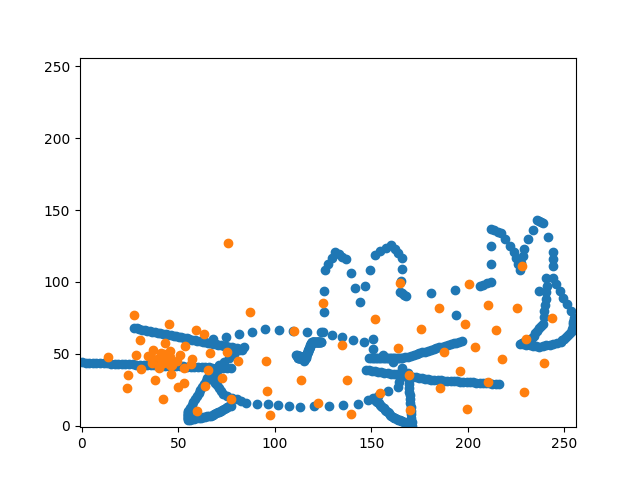
\includegraphics[keepaspectratio, scale=0.45]{draw-forecast/fig/pointnet_output2.png}
    \subcaption{Perplexityにより質を改善したデータ}
    \label{fig:pointnet_output_perplexity}
  \end{minipage}
  \caption{青が完成形・オレンジがモデルの出力}
\end{figure}

Quick Draw!\cite{quickdraw} のデータセットは、世界中のユーザーから集めたデータであるため質のばらつきが大きく、人間でも判別がつかないようなデータも多く含まれていました。このため、まずデータの選別を行う必要があると考え、PointNet\cite{pointnet}を用いたクラス分類モデルを構築し、Perplexityを用いて低品質なデータを除外しました。データセットを半分に削減した結果、図\ref{fig:pointnet_output_perplexity}のように生成された点群に多少のまとまりが見られるようになりましたが、それでも絵としての復元には至りませんでした。

\subsection{失敗した要因}
クラスの分類タスクでは、PointNet\cite{pointnet}を用いたモデルが80\%以上の精度を達成したことから、点群によるアプローチが上手くいかなかった原因はエンコーダではなくデコーダにあると考えられます。固定長を一度に出力する手法では点群の順序に依存しない特性、逐次生成ではデータ内の描き順のばらつきによる一貫性の欠如が、上手く生成できなかった原因であると思います。

\section{時系列データ}
Quick Draw!\cite{quickdraw}のデータは、点の座標の時系列データとして表現されているため、まず単純なTransformerを用いて次の点を予測する学習を試みましたが、意味のある出力を得ることはできませんでした。

Quick Draw!\cite{quickdraw}のデータセットを用いた線画の生成に関する論文として、sketchRNN\cite{sketchRNN}というモデルがあり、Googleが開発した初めのモデルとなります。sketchRNN\cite{sketchRNN}は、エンコーダに双方向性LSTMを採用し、入力データを潜在空間に埋め込んだ後、デコーダとしてLSTMを用いて復元する、VAEに基づいた生成モデルです。
\begin{figure}[h]
  \centering
  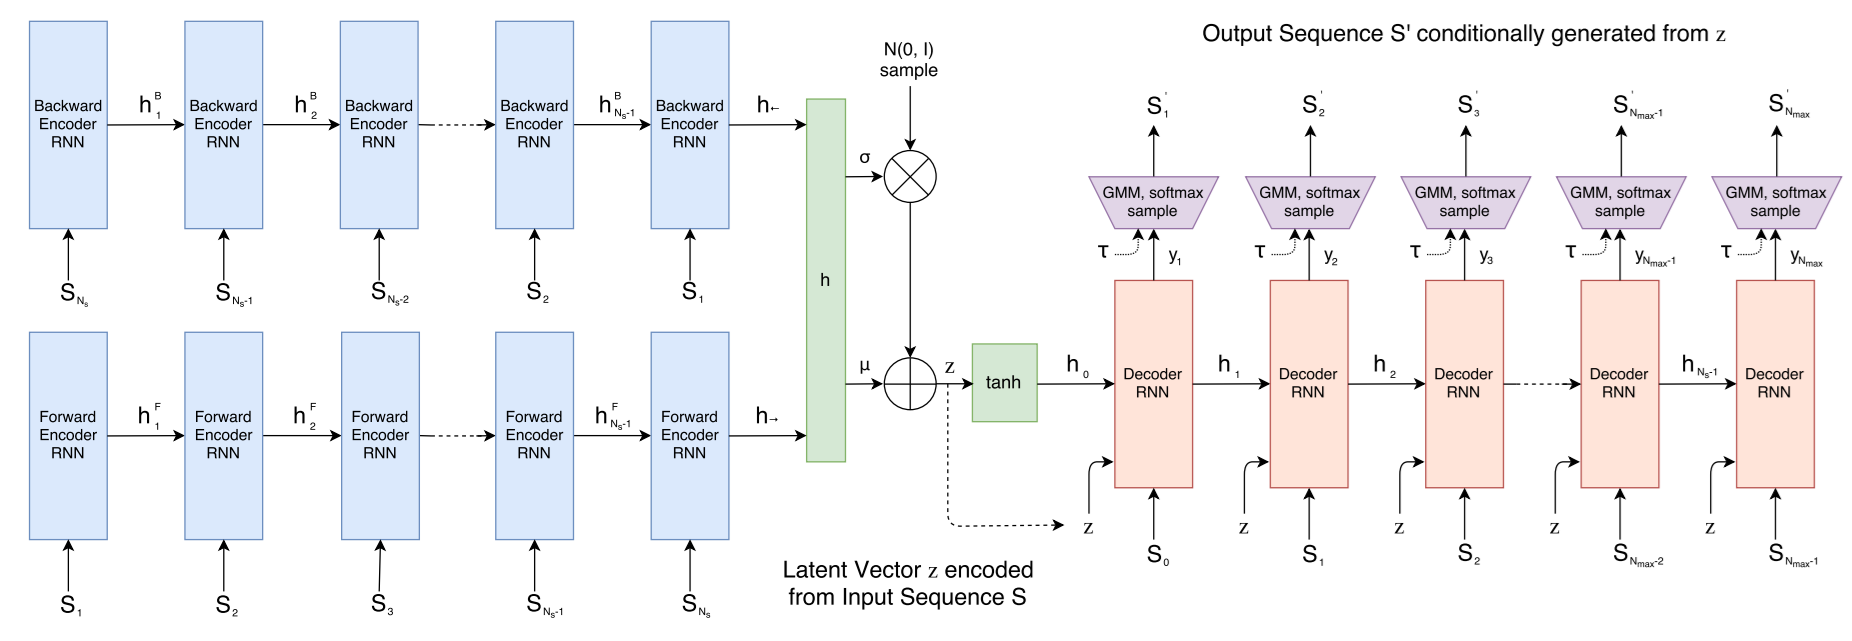
\includegraphics[scale=0.45]{draw-forecast/fig/sketchrnn.png}
  \caption{SketchRNN}
  \label{fig:sketchrnn}
\end{figure}
データの前処理として、直接的な座標ではなく前の点からの差分の座標を使用し、「ペンを下ろしている」・「ストロークの終わり」・「絵の終わり」の3つの状態を表すワンホットベクトルを合わせた5次元の系列データで学習を行います。出力については、座標の差分の分布に混合正規分布を仮定し、サンプリングによって次点の予測を行います。混合正規分布を用いることで、複数の書き順が存在することによって学習が不安定化する問題点を解決しています。ただし、複数のクラスを1つのモデルで同時に学習させることは難しく、1クラス毎に個別のモデルを学習させる必要があります。

また、LSTMではなくTransformerを用いたsketchformer\cite{sketchformer}というモデルもあり、こちらのモデルではsketchRNN\cite{sketchRNN}とは異なり、単一モデルで複数クラス全ての学習を同時に行っても精度よく生成することが可能となります。しかし、論文の内容を再現してみても学習が上手く進まず、時間の制約から本プロジェクトでは使用することができませんでした。

\section{終わりに}

今回は、途中まで描かれた絵から完成形を描くAIの作成に挑戦しましたが、時間の制約と実力不足により、最終的には初期の線画生成モデルであるSketchRNN\cite{sketchRNN}を採用する形となり、Transformerを用いたsketchformer\cite{sketchformer}などの新しいモデルや、独自の工夫を加えた実験を十分に行うことができずに終わってしまいました。今後は、sketchformer\cite{sketchformer}の実装や、Diffusionモデルなどの様々な生成手法を取り入れた実験を行い、より完成度の高いモデルを作成していきたいと思います。
